\documentclass[main.tex]{subfiles}

\begin{document}

\section{Aufgabe 5}
Gegeben ist die Funktion
\begin{equation*}
    f(x) =\frac{1}{x} + 2
\end{equation*}

\begin{enumerate}
    \item[(a)] Zeigen Sie, dass die Funktion auf dem Intervall $[2;5]$ die Voraussetzungen des Fixpunktsatzes erfüllt.
    \item[(b)] Mit dem Startpunkt $x_{0} = 3$ berechnen Sie mit der a-priori-Abschätzung die notwendige Anzahl Iterationen, um den Fixpunkt mit der Genauigkeit $\epsilon =\frac{1}{1.000}$ zu berechnen.
    \item[(c)] Mit demselben Startpunkt und derselben verlangten Genauigkeit, berechnen Sie die Iterationen, bis mit der a-posteriori Abschätzung die Genauigkeit erreicht ist.
\end{enumerate}

Sie dürfen die Monotonie der Funktion ausnutzen.

\subsection{Lösung 5}

\begin{figure}[ht]
	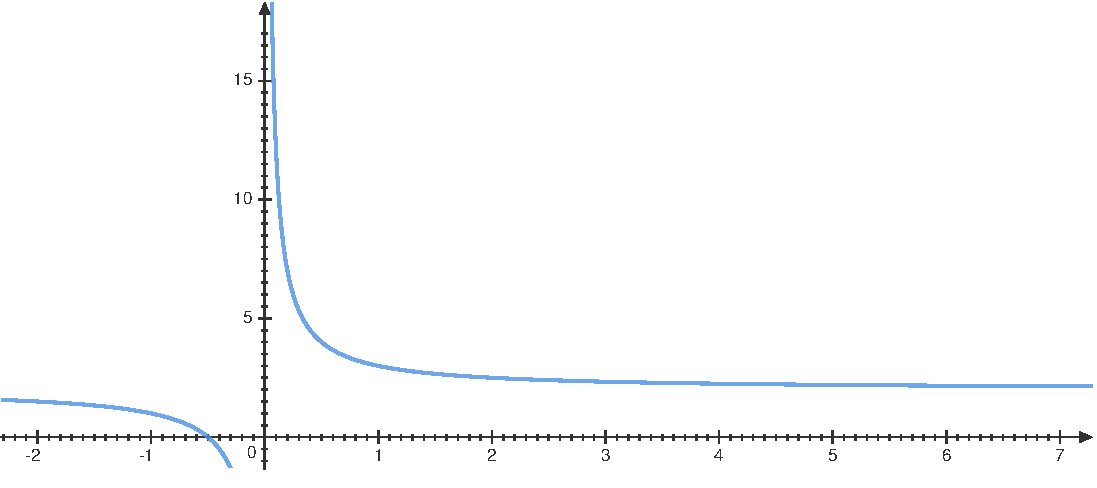
\includegraphics[width=\linewidth]{fig-5.pdf}
	\caption{Graph von $f(x)$}
\end{figure}

\subsubsection{Lösung 5a}

\begin{quote}
    Fixpunktsatz: Sei $f:[ a,b]\rightarrow [ c,d]$ stetig mit $[ c,d] \subset [ a,b]$ (selbstkontrahierend), dann existiert ein Fixpunkt $u=f(u)$.
    \textit{(Schelthoff, S. 157 Satz 143)}\footnote{Schelthoff, Christof (2018): MATSE-MATIK.\@ Analysis 1, 6. Auflage, Aachen, Shaker Verlag.}
\end{quote}

$f(x) =\frac{1}{x}$ ist bekanntermaßen stetig für $x\neq 0$ und da die Definitionslücke nicht in dem untersuchten Intervall enthalten ist $0\notin [ 2;5]$ ist die Funktion in dem Intervall stetig.

Die Funktion bildet das Intervall $\displaystyle {\textstyle [ 2;5]}$ auf das Intervall${\textstyle \left[\frac{5}{2} ;\frac{11}{5}\right]}$ ab 
\begin{equation*}
    {\textstyle f:[ 2;5] \ \rightarrow \left[\frac{5}{2} ;\frac{11}{5}\right]}
\end{equation*}
und der Wertebereich ist Teilmenge des Definitionsbereichs
\begin{equation*}
    {\textstyle \left[\frac{5}{2} ;\frac{11}{5}\right] \subset [ 2;5] \ \checked }
\end{equation*}

also exisiter ein Fixpunkt.

\subsubsection{Lösung 5b}

Eine Funktion $f:D\rightarrow \mathbb{R}$ ist Lipschitz-stetig in einem Punkt $x_{0} \in D$, wenn gilt
\begin{equation*}
    \exists L\geq 0\forall x,x_{0} \in D:| f( x) -f( x_{0})| \leq L\cdot | x-x_{0}| \text{.}
\end{equation*}
Daraus folgt für die Lipschitz-Konstante $L$
\begin{equation*}
    L\geq \frac{| f( x) -f( x_{0})| }{| x-x_{0}| }
\end{equation*}
Für die gegebene Funktion bedeutet das:
\begin{equation*}
    \begin{array}{ c c l }
    L & \geq  & \frac{\left| \left(\frac{1}{x} +2\right) -\left(\frac{1}{x_{0}} +2\right)\right| }{| x-x_{0}| }\\
    & = & \frac{\left| \frac{1}{x} -\frac{1}{x_{0}}\right| }{| x-x_{0}| }\\
    & = & \frac{\frac{| x_{0} -x| }{x\cdot x_{0}}}{| x-x_{0}| }\\
    & = & \frac{| x_{0} -x| }{x\cdot x_{0} \cdot | x-x_{0}| }\\
    & = & \frac{1}{x\cdot x_{0}}
    \end{array}
\end{equation*}
Die Fixpunkt-Iteration zur numerische Annäherung an Fixpunkt $x_{n+1}$ lautet
\begin{equation*}
    x_{n+1} =f( x_{n}) =\frac{1}{x_{n}} +2
\end{equation*}
Diese ist gleichmäßig stetig auf dem Intervall $\displaystyle [ 2;5]$ mit
\begin{equation*}
    \left| \left(\frac{1}{x} +2\right) -\left(\frac{1}{x_{0}} +2\right)\right| =\left| \frac{1}{x} -\frac{1}{x_{0}}\right| \leq \left| \frac{x_{0} -x}{x\cdot x_{0}}\right| \leq \frac{1}{2\cdot 2}| x-x_{0}| 
\end{equation*}
und die Abbildung ist kontrahierend. Weiterhin ist mit $x_{0} =3$ dann $x_{1} =f( 3) =\frac{7}{3}$, also ist
\begin{equation*}
    | x_{1} -x_{0}| =\left| \frac{7}{3} -\frac{9}{3}\right| =\frac{2}{3}\text{.}
\end{equation*}

Der Fixpunkt soll mit einer Genauigkeit von $\epsilon =\frac{1}{1.000}$ berechnet werden.

Eine a-priori Abschätzung erfolgt für den Fehler $\left| x_{n} -x^{*}\right| $, wobei $x_{n}$ ist der Fixpunkt mit der Genauigkeit $\epsilon $ und $x^{*}$ der eigentlich Fixpunkt ist, nach folgender Definition (Schelthoff, S. 157 Satz 144):
\begin{equation*}
    \left| x_{n} -x^{*}\right| \leq \frac{L^{n}}{1-L} \cdotp | x_{1} -x_{0}| < \epsilon \text{mit} x_{0} \in [a;b] ,\ x_{1} =f( x_{0})\text{.}
\end{equation*}

Mit $L=\frac{1}{4}$ ergibt sich nach der folgenden Umformung für die Anzahl der Iterationen:
\begin{equation*}
    \begin{array}{ c c c l }
        & L^{n} & <  & \frac{\epsilon \cdot ( 1-L)}{| x_{1} -x_{0}| }\\
        \Leftrightarrow  & n &  > & \frac{\ln\left(\frac{| x_{1} -x_{0}| }{\epsilon \cdot ( 1-L)}\right)}{\ln\left(\frac{1}{L}\right)}\\
        \equiv  & n &  > & \frac{\ln\left(\frac{\frac{2}{3}}{\frac{1}{1.000} \cdot \left( 1-\frac{1}{4}\right)}\right)}{\ln( 4)}\\
        &  & = & \frac{\ln\left(\frac{2\cdot 1.000}{3} \cdot \frac{4}{3}\right)}{\ln( 4)}\\
        &  & = & \frac{\ln\left(\frac{2\cdot 1.000\cdot 4}{3\cdot 3}\right)}{\ln( 4)}\\
        &  & = & \frac{\ln\left(\frac{8.000}{9}\right)}{\ln( 4)}\\
        &  & \approx  & 4,897\dotsc 
    \end{array}
\end{equation*}

Damit ist $n_{0} =5$ und die Berechnung des Fixpunktes in der gewünschten Genauigkeit nach 5 Iterationen erreicht.

\subsubsection{Lösung 5c}

Für die a-posteriori Abschätzung gilt analog $\left| x_{n} -x^{*}\right| \leq \frac{1}{1-L} \cdotp | x_{n} -x_{n-1}| < \epsilon $ und bleibt dem Leser als Aufgabe selbst überlassen.


\end{document}
